% CoScientist demo paper, AAAI-27 Demonstrations. 2 pages + 1 page of references.
% Build: pdflatex main && bibtex main && pdflatex main && pdflatex main
% Single-blind: author names stay. Places that wait for the main run are marked TODO(run).

\documentclass[letterpaper]{article} % DO NOT CHANGE THIS
\usepackage{aaai2027}  % DO NOT CHANGE THIS
\usepackage[hyphens]{url}  % DO NOT CHANGE THIS
\usepackage{graphicx} % DO NOT CHANGE THIS
\urlstyle{rm} % DO NOT CHANGE THIS
\def\UrlFont{\rm}  % DO NOT CHANGE THIS
\usepackage{natbib}  % DO NOT CHANGE THIS AND DO NOT ADD ANY OPTIONS TO IT
\usepackage{caption} % DO NOT CHANGE THIS AND DO NOT ADD ANY OPTIONS TO IT
\frenchspacing  % DO NOT CHANGE THIS
\DeclareCaptionStyle{ruled}{labelfont=normalfont,labelsep=colon,strut=off} % DO NOT CHANGE THIS
\usepackage{booktabs}

\pdfinfo{
/TemplateVersion (2027.1)
}

\setcounter{secnumdepth}{0}

\title{CoScientist: Autonomous Research Runs That Leave\\Reusable Tool Servers Behind}

% Author order is provisional.
\author{
    Stanislav Chumakov,
    Nargiza Amerkhanova,
    Gleb Solovev,
    Rodion Golovinsky,
    Denis Chistyakov,
    Evgenii Klokov,
    Ivan Guryev,
    Anna Kalyuzhnaya,
    Nikolay Nikitin
}
\affiliations{
    ITMO University, Saint Petersburg, Russia\\
    stas1f1@gmail.com
}

\begin{document}

\maketitle

\begin{abstract}
Large language model systems can carry out separate stages of scientific and
engineering research, yet the code, environments, and intermediate results they
produce rarely outlive the session that created them. We present CoScientist, a
multi-agent system that plans a study in a typed research graph, searches the
literature, runs experiments, and, through its Alembic module, converts
scientific repositories into validated Model Context Protocol (MCP) servers
shared in an open Docker Hub catalogue. An agent looks for a tool locally, then
in the catalogue, and converts a repository only when neither has it. We
demonstrate the system on an industrial task, the computational design of tyre
rubber compounds. The system finds which published methods still run, tests them on 3,774
patent recipes under a split that holds out whole patents, refutes its own
benchmark hypothesis, and leaves the working tools, the session, and the graph
behind; a second session answers a follow-up question in four minutes with a
server the first one built.
\end{abstract}

\begin{links}
    \link{Tool catalogue}{https://hub.docker.com/u/peanutbuttermilk}
    \link{Code}{https://github.com/aimclub/CoScientist}
    \link{Video}{TODO(video)}
\end{links}

\section{Introduction}

Agentic systems now cover most stages of a computational study: they propose
hypotheses \citep{gottweis2026coscientist}, run experiments
\citep{lu2026aiscientist}, and analyse data over long horizons
\citep{mitchener2025kosmos}. Such a run leaves a report, code, and logs; the environment in which a
published method finally ran is rebuilt by the next run.

Research code makes this costly: of eight published methods in our case study,
four run.

We present \textbf{CoScientist}, in which a research run (i) keeps questions,
hypotheses, evidence, and artefacts in a typed research graph, (ii) obtains
tools by reuse first: a local server, then a public catalogue, then a
conversion of the repository, and (iii) leaves three artefacts for a follow-up
study: runnable tool servers, an exported session, and the graph.

\section{Related Work}

AI-scientist systems end a run with a paper, code, and logs
\citep{lu2026aiscientist,schmidgall2025agentlab}, ranked hypotheses
\citep{gottweis2026coscientist}, or a report that cites code and literature
\citep{mitchener2025kosmos}.
Repository-to-tool systems produce a function
\citep{wolflein2025toolmaker} or an MCP server
\citep{ouyang2026code2mcp,miao2026paper2agent,di2026toolrosella}. DFAgent builds a governed catalogue of MCP tools from logged code
\citep{gantayat2026dfagent}; ToolSmith generates and validates enterprise
tools \citep{vakudavathu2026toolsmith}. Engineering agents exist for mechanics and materials
\citep{ni2024mechagents,kang2024chatmof}. CoScientist combines these lines: conversion happens inside a research run,
its product is a runnable image in a public catalogue that grows as a
by-product of agent work, and servers, session, and graph together let a study
continue after a negative result. Earlier versions targeted chemistry \citep{solovev2025chemcoscientist,solovev2025madd}.

\section{System Overview}

\begin{figure*}[t]
  \centering
  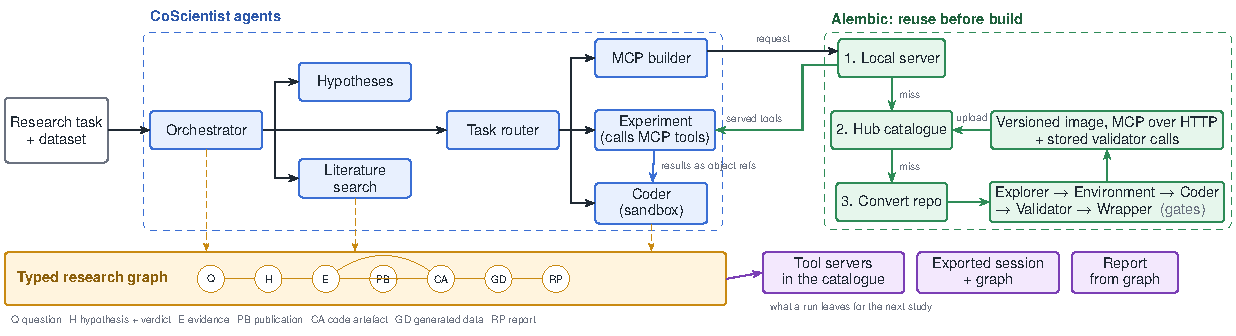
\includegraphics[width=0.94\textwidth]{figures/architecture.pdf}
  % TODO(figure): optional screenshots of the catalogue page and the tyre graph next to it.
  \caption{CoScientist. Agents write questions, hypotheses, evidence, and
  artefacts to one typed research graph (dashed). A tool from a repository is
  looked up on the host, then in the public catalogue, and built by Alembic only
  when both miss. A run ends with tool servers, an exported session with the
  graph, and a report generated from the graph.}
  \label{fig:system}
\end{figure*}

\textbf{Research graph.} An orchestrator frames the request as a research
question and delegates by the kind of work. All agents write to one typed
graph \citep{coscientist2026repo}: questions, hypotheses, evidence, publications,
code artefacts, generated data, and reports, with typed edges and per-agent write permissions; a background validator sets
hypothesis verdicts, and the final report is generated from the graph.

\textbf{Agents.} A research agent searches the web and OpenAlex; a coder agent
collects data and trains models in a sandbox; ready tools are found by
retrieval over a catalogue of MCP servers and called by an experiment agent,
with large results passed as object-store references.

\textbf{Alembic.} Given a repository URL, Alembic runs five stages in a
container: it proposes tools from the repository's documentation, builds the
repository environment apart from the server environment, writes each tool as
a function with tests, calls every tool, and renders an MCP server. Gates check symbols, imports, and tests between stages; every validator call
is stored with its arguments and result.

\textbf{Reuse before build.} A tool request goes through a cascade: a server
on the host, then an image in the public Docker Hub namespace, then a
conversion. An automatic upload never replaces a build with more passing tools. The catalogue holds 19 servers from chemistry,
materials, climate, geoscience, physiology, cognitive science, and
biomedical imaging; pulling one takes no model calls.

\section{Case Study: Tyre Rubber Compounds}

Tyre producers keep recipes secret. We asked CoScientist whether published
methods and open data allow a recipe to be designed computationally.
The prompt gives the goal, 3,774 compounds parsed from 337 patents (recipe in
phr, ingredient grades, process parameters, twelve properties), and eight
published methods. It names neither MCP nor Alembic. The model is
GLM-5.3. Table~\ref{tab:runs} sets the run against a coding agent (opencode) on the
same prompt and model, and against a chemist's manual study.

\textbf{Which methods run.} The system installed and ran each method. Four of seven run: polyBERT \citep{kuenneth2023polybert},
PolymerGNN \citep{queen2023polymergnn}, TransPolymer, and the Wan et al.
models \citep{wan2024coco}, whose Keras weights the system found in a
repository our chemist had not run.
The rest \citep{hu2024jmi,roychoudhury2025jrr} publish neither code nor data.

\begin{table}[t]
\centering
\footnotesize
\setlength{\tabcolsep}{3pt}
\begin{tabular}{@{}lrrr@{}}
\toprule
 & CoScientist & opencode & manual \\
\midrule
Wall time                          & 105 min & 60 min & weeks \\
Cost, USD                          & 3.4 & 6.3 & -- \\
Methods verified to run            & 4 of 7 & 2 of 9 & 3 of 9 \\
$R^2$ Mooney, random / patent   & 0.8 / $-$0.3 & 0.8 / 0.1 & 0.7 / 0.0 \\
$R^2$ M300, random / patent     & 0.9 / 0.0 & 0.9 / 0.4 & 0.8 / 0.3 \\
Left behind & graph, servers & scripts & repo \\
\bottomrule
\end{tabular}
\caption{Two agent runs on the same prompt and model, and a chemist's prior
manual study of the same data. $R^2$ is five-fold with each study's own
features; the manual by-patent value is our re-evaluation of its model.}
\label{tab:runs}
\end{table}

\textbf{Forward models.} With a random split the recipe predicts most
properties, and with whole patents held out $R^2$ falls to about zero in both
runs. The system traced this to one-hot ingredient grades, which encode patent
families, so a random split rewards memorising near copies. The
manual study grouped folds by exact recipe, which keeps such copies on both
sides, and reported $R^2$ of 0.7. Adding polyBERT or TransPolymer fingerprints
gives no significant change in a paired test ($p>0.27$). The system refuted its
benchmark hypothesis, postponed three follow-up hypotheses, and proposed five
candidate recipes from an NSGA-II search over an ensemble, noting that the
uncertainty is optimistic (coverage 0.39). The baseline reached a comparable
analysis and added a finding: the strongest Mooney predictor is a measured
property of the raw elastomer, unavailable at design time.

\textbf{What remains.} The baseline leaves scripts, clones, and a report on
one machine. CoScientist leaves a graph of 40 nodes with verdicts, an exported
session (0.5\,MB), and, on a one-line request at the end of the session, two
servers built by Alembic from the methods that ran: the Wan et al. models (4
tools) and TransPolymer (5 tools), every tool passing its tests and live calls;
both are in the catalogue. No human step was needed: the Wan repository holds no
code, only three Keras files, so Alembic read the network structure from the
HDF5 itself and pinned TensorFlow 2.15 to load the 2020 weights; for
TransPolymer it fetched 329\,MB of LFS weights without git-lfs and pinned a
transformers version that still has the API the code imports, which the
baseline solved by rewriting the tokeniser by hand. PolymerGNN's requirements
name versions that do not exist; Alembic substituted working ones.
In a repeat experiment, a new session asked for the properties of one
candidate recipe; the agent found the Wan server in the catalogue and answered
in four minutes for \$0.14. The polyBERT server's
blend fingerprints match to six decimals values computed by hand.

\section{Demonstration and Limitations}

Visitors pull a server from the catalogue and call a tool from the browser,
browse the tyre session (hypotheses, verdicts, evidence, tool calls), and see
the follow-up session answer with a catalogue server. CoScientist treats the tools and the
record of a study as its products: the next tyre study starts from running
servers and a graph of what was tried. Limits: internal validation, one case,
analysis on par with a coding agent.

\bibliography{references}

\end{document}
